\section{Evaluation}
\label{sec:eval}

\iffalse
% On 8/11, WRW confirms these are all done.
\GS{\sout{we had this part in rebuttal: "We will make available supplementary
materials, including (a) the human study website itself as well as the stimuli,
(b) the source code, and (c) a demonstration website at which arbitrary programs
can be passed to our algorithm and the output can be observed."}}
\fi

We have implemented our approach in \toolname: a system for repairing parse
errors for \python in its entirety. The code for \toolname is publicly available
at \url{https://github.com/gsakkas/seq2parse} and a simplified online
demonstration is available at \url{http://seq2parse.goto.ucsd.edu/index.html}.
Next, we describe our implementation and an evaluation that addresses four
questions:

\begin{itemize}
    \item \textbf{RQ1}: How \emph{accurate} are \toolname's predicted error production rules?
                        (\S~\ref{sec:eval:accuracy})
    \item \textbf{RQ2}: How \emph{precisely} can \toolname repair parse errors?
                        (\S~\ref{sec:eval:precise})
    \item \textbf{RQ3}: How \emph{efficiently} can \toolname repair parse errors?
                        (\S~\ref{sec:eval:efficiency})
    \item \textbf{RQ4}: How \emph{useful} are \toolname's suggested repairs?
                        (\S~\ref{sec:eval:useful})
\end{itemize}

% \subsection{Implementation} \label{sec:eval:gen_method}

\mypara{Training Dataset}
For our evaluation, we use the same \python dataset that we used in our error
data analysis in \autoref{sec:error-analysis} gathered from
PythonTutor.com~\citep{Guo2013} between the years 2017 and 2018. The dataset has
more than 1,100,000 usable erroneous Python programs and their respective fixes.
The programs have an average length of \emph{87 tokens}, while the abstracted
token sequences have a much shorter average of \emph{43 tokens}. We choose
15,000 random programs from the dataset for all our tests, and the rest we use
as our training set.

We first learn a PCFG on the training set of fixed programs to learn the
probabilities for each production rule in the \emph{full \python grammar}.
\toolname then extracts the abstracted token sequences for all programs in the
training set. Next, while the full \python grammar has \emph{455 possible
terminal error production rules}, in reality, only \emph{340 error rules} are
ever used in our dataset and are assigned as \emph{labels}. We arrive at this
set of error rules by parsing all the erroneous programs in the training set
with the ECE-Parser and the ``diff'' error rules, as described in
\autoref{sec:whole-system:error-rules}.

\mypara{Transformer Classifier}
\toolname's error rule prediction uses a Transformer classifier with \emph{six}
transformer blocks, that each has a fully-connected hidden layer of 256 neurons
and 12 attention heads. The output of the transformer blocks is then connected
to a \dnn-based classifier with \emph{two} fully-connected hidden layers of 256
and 128 neurons respectively. The neurons use rectified linear units (ReLU) as
their activation function, while the output layer uses the sigmoid function for
each class. Additionally, there are \emph{two input embedding layers} of a
length of 128 units, one for input tokens and one for their positions in the
sequence. We also limit the input abstracted token sequences to a length of 128
tokens, which covers $95.7\%$ of the training set, without the need of pruning
them. Finally, the Transformer classifier was trained using an \textsc{Adam}
optimizer \citep{Kingma2014-ng}, a variant of stochastic gradient descent, on
NVIDIA GeForce RTX 3080 Ti for a total of 50 epochs.

\subsection{RQ1: Accuracy}
\label{sec:eval:accuracy}

% colors from http://colorbrewer2.org/?type=sequential&scheme=Blues&n=3
\definecolor{blue1}{HTML}{DEEBF7}
\definecolor{blue2}{HTML}{9ECAE1}
\definecolor{blue3}{HTML}{3182BD}
\definecolor{green1}{HTML}{E5F5E0}
\definecolor{green2}{HTML}{A1D99B}
\definecolor{green3}{HTML}{31A354}

\begin{figure}[t]
  % \begin{minipage}[c]{0.49\linewidth}
    \centering
    \resizebox{0.6\linewidth}{!}{
      \Large
      \begin{tikzpicture}
      \begin{axis}[
        ybar stacked,
        width=1.1\linewidth,
        height=11cm,
        % title={Accuracy of Repair Template Prediction},
        ylabel={Prediction Accuracy (\%)},
        bar width=1cm,
        ymin=0.0,
        ymax=101.0,
        ytick={0.0, 10.0, 20.0, 30.0, 40.0, 50.0, 60.0, 70.0, 80.0, 90.0, 100.0},
        yticklabel={\pgfmathparse{\tick}\pgfmathprintnumber{\pgfmathresult}},
        ytick style={draw=none},
        ymajorgrids = true,
        symbolic x coords={original, abstracted, abstracted-best},
        enlarge x limits=0.3,
        xtick=data,
        xtick style={draw=none},
        xticklabels={\textsc{Original}\xspace, \textsc{Abstracted}\xspace, \textsc{Threshold}\xspace},
        %x tick label style={rotate=45, anchor=north east},
        % x tick label style={font=\small},
        % y tick label style={font=\small},
        reverse legend,
        % transpose legend,
        legend style={legend pos = north east, legend columns=4, font=\small},
      ]

      \addplot[draw=black, fill=blue2, bar shift=-.501cm, postaction= { pattern=dots }] coordinates {(original, 0.0) (abstracted, 0.0) (abstracted-best, 79.28025102961365)};

      \resetstackedplots

      \addplot[draw=black, fill=green2, bar shift=.501cm, postaction= { pattern=dots }] coordinates {(original, 0.0) (abstracted, 0.0) (abstracted-best, 69.82968369829683)};

      \resetstackedplots

      \addplot[draw=black, fill=green1, bar shift=.501cm] coordinates {(original, 12.875536480686696) (abstracted, 58.394160583941606) (abstracted-best, 0.0)};
      \addlegendentry{Top-10}
      \addplot[draw=black, fill=green2, bar shift=.501cm] coordinates {(original, 20.100143061516448) (abstracted, 14.922952149229523) (abstracted-best, 0.0)};
      \addlegendentry{Top-20}
      \addplot[draw=black, fill=green3, bar shift=.501cm] coordinates {(original, 31.974248927038623) (abstracted, 15.49067315490673) (abstracted-best, 0.0)};
      \addlegendentry{Top-50}
      \addlegendimage{empty legend}
      \addlegendentry{Rare:}

      \resetstackedplots

      \addplot[draw=black, fill=blue1, bar shift=-.501cm] coordinates {(original, 56.712132089016514) (abstracted, 72.11217885859972) (abstracted-best, 0.0)};
      \addlegendentry{Top-10}
      \addplot[draw=black, fill=blue2, bar shift=-.501cm] coordinates {(original, 11.769733018835673) (abstracted, 9.335163757599531) (abstracted-best, 0.0)};
      \addlegendentry{Top-20}
      \addplot[draw=black, fill=blue3, bar shift=-.501cm] coordinates {(original, 18.65107852186101) (abstracted, 11.253840622344256) (abstracted-best, 0.0)};
      \addlegendentry{Top-50}
      \addlegendimage{empty legend}
      \addlegendentry{All:}

      \end{axis}
      \end{tikzpicture}
    }
    \caption{
      Results of our error production rule prediction classifiers for the simple original token sequences and their abstracted versions using the PCFG.
    }
    \label{fig:accuracy-results}
  % \end{minipage}
  % \begin{minipage}[c]{0.49\linewidth}
  %   \centering
  %   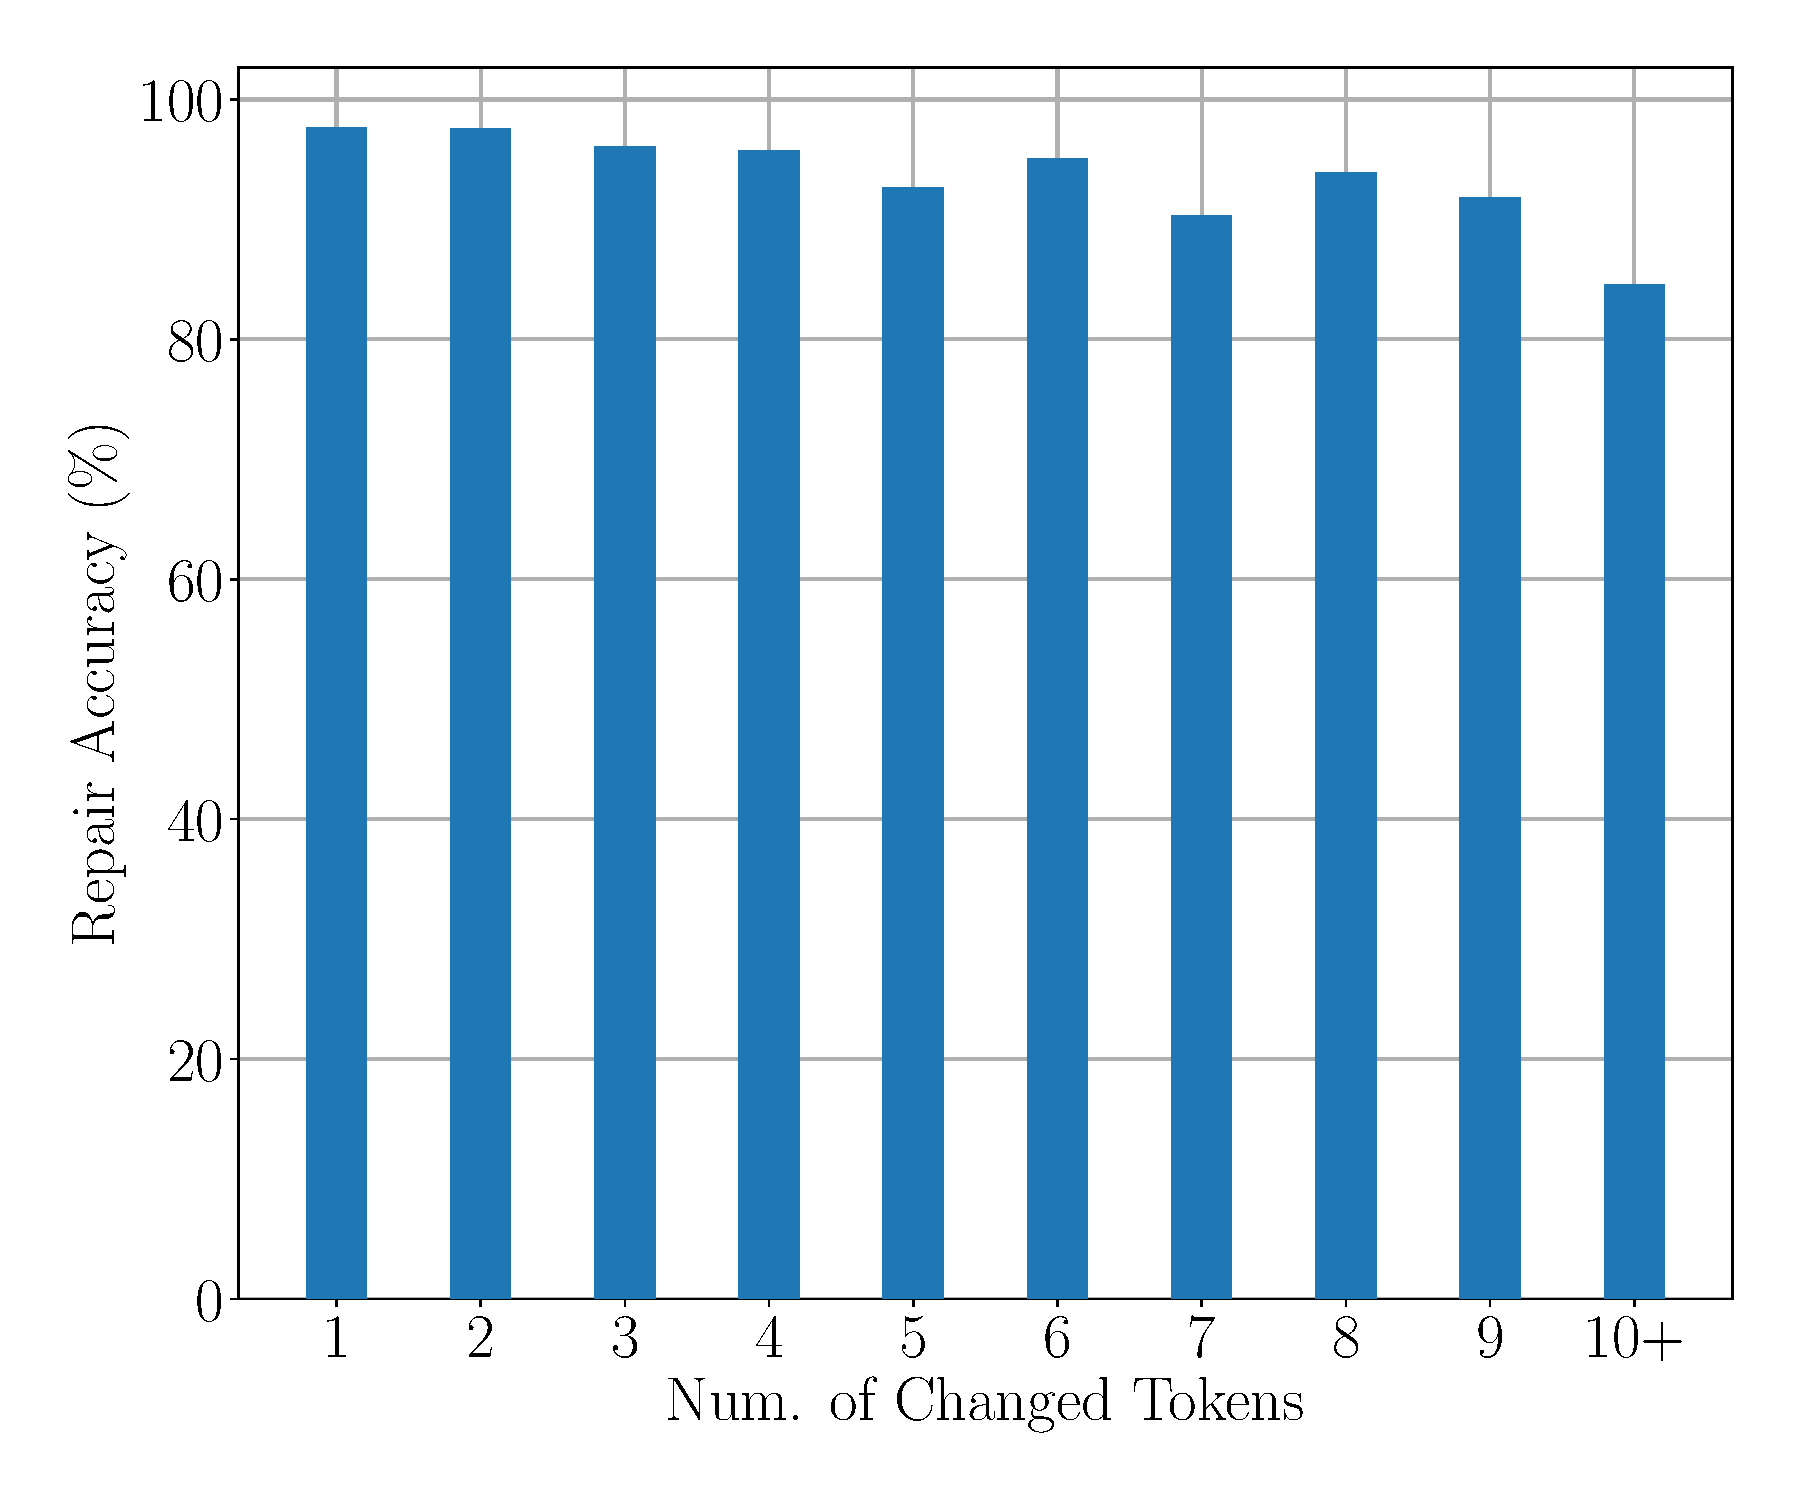
\includegraphics[width=\linewidth]{accuracy-per-change.pdf}
  %   \caption{The repair accuracy for the number of edits needed by the user to repair.}
  %   \label{fig:accuracies-per-changes}
  % \end{minipage}
\end{figure}


\autoref{fig:accuracy-results} shows the accuracy results of our error
production rule prediction experiments. The y-axis describes the
\emph{prediction accuracy}, \ie the fraction of test programs for which the
correct \emph{full set} of error rules to repair the program (extracted from
the user fix) was predicted in the top-K sorted rules.
% \GS{\sout{Accuracy is computed by ...}}
%
The \textsc{Original} version of our transformer classifier does not consider
the abstracted token sequences and used the full \textsc{Original} token
sequences, whose results are presented in the first two bars of
\autoref{fig:accuracy-results}. The next four bars show our final results using
the \textsc{Abstracted} token sequences to train the classifier with
\textsc{NoPCFG} and with fully \textsc{Abstracted} sequences. Finally, the last
two dotted bars show the results for when a probability \textsc{Threshold} is
set in order to select the predicted error rules (instead of picking the static
top-K ones) but using again the \textsc{Abstracted} sequences as input. The
predicted error rule set ranges between 1--20 elements.

The blue bars show the accuracy on the full test set of \textsc{All} 15,000 test
programs, while the green bars show the results on a subset of \textsc{Rare}
programs, \ie programs that did not include any of the 50 most popular error
rules. The \textsc{Rare} programs account for 1233 programs, roughly 8\% of our
test set.

The \textsc{Original} predictor, even with the Top-50 predicted error rules, is
less accurate than the Top-20 predictions of the \textsc{Abstracted}, with an
accuracy of 87.13\%, which drops to 68.48\% and 56.71\% respectively for the
Top-20 and Top-10 predictions. The \textsc{Abstracted} predictor significantly
outperforms the \textsc{Original} predictor with a 72.11\% Top-10 accuracy,
81.45\% Top-20 accuracy and 92.70\% Top-50 accuracy.

The \textsc{Threshold} predictions are almost as accurate as the
\textsc{Abstracted} Top-20 predictions with an accuracy of 79.28\% and a median
number of selected error rules of 14 (average 14.1). This could potentially mean
that this predictor is a valid alternative for the static Top-20 predictions.

\GS{Should we mention sensitivity anywhere else, before this?} The classifiers
are also not very \emph{sensitive} in the PCFG probabilities used during
abstraction, as shown in the accuracy of the \textsc{NoPCFG} predictor. The
\textsc{NoPCFG} predictor has almost 2\% less Top-10 and Top-20 accuracy,
70.94\% and 80.69\% respectively, and less than 1\% for Top-50 predictions, with
92.11\%.

Finally, we observe that our \textsc{Abstracted} classifiers generalize
efficiently for our dataset of erroneous \python programs and are almost as
accurate for the \textsc{Rare} programs as the rest of the dataset with a
73.32\% Top-20 accuracy (88.81\% Top-50 accuracy). The same holds for the
\textsc{Threshold} predictions with a 69.83\% \textsc{Rare} accuracy. The
\textsc{NoPCFG} also has a drop of more than 2\% accuracy, with a 71.29\% Top-20
accuracy (86.29\% Top-50 accuracy).

\begin{framed}
  \noindent \toolname's transformer classifier learns to encode programs with
  syntax errors and select candidate error production rules for them
  effectively, yielding \emph{high accuracies}. By abstracting the tokens
  sequences, \toolname is able to \emph{generalize} better and make more
  accurate predictions with a \emph{81.45\% Top-20 accuracy}.
\end{framed}


\subsection{RQ2: Repaired Program Preciseness}
\label{sec:eval:precise}


\iffalse
% On 8/11, WRW confirms these are all done.
\GS{\sout{TODO: We had this part in rebuttal: "We will augment the text in
Section 7.2 to explain that the MinimumCost version of Seq2Parse only retains
the top \#1 (minimum cost) repair, resulting in a more efficient parser, unlike
AllParses, which is slower but retains all possible repairs and thus obtains a
higher accuracy (as shown in Section 7.3)"}}

\GS{\sout{TODO: Clarify on the difference of the 3 approaches better. why they are
allowed different numbers of edits. "We will elaborate that the maximum number
of edits was selected to provide a uniform (wall clock) run time for the
algorithms (e.g., since MinimumCost is faster than AllParses)."}}
\fi

Next we evaluate \toolname's end-to-end accuracy and preciseness when
restricting \toolname's parsing time to \emph{5 minutes} and run our experiments
on the 15,000-program test set. Additionally, we use here the highest-performing
transformer classifiers, \ie the \textsc{Abstracted}, \textsc{NoPCFG} and
\textsc{Threshold} classifiers.

We compare \emph{three versions} of our \toolname implementation
(\textsc{AllParses}, \textsc{MinimumCost} and \textsc{Threshold}) against two
versions of the ECE-Parser with a static selection of the 20 and 50 most popular
error production rules in our training set. We make this choice because we
observe that the 50 most popular error rules are used as labels for as much as
\emph{86\%} of the training set. For the \textsc{AllParses},
\textsc{MinimumCost} and \textsc{Threshold} versions, we run our experiments for
the \textsc{Abstracted} and \textsc{NoPCFG} classifier predictions.

Our \textsc{AllParses} and \textsc{MinimumCost} ECE-Parsers both use the
\emph{Top-20 predictions} from our \textsc{Abstracted} classifier to parse and
repair buggy programs. The \textsc{AllParses} ECE-Parser keeps internally
\emph{all possible states} that arise from using the predicted error rules
similarly to the original ECE-Parser described by \citet{Aho_1972}. We use a
maximum repair cost of 2 edits (\ie, a maximum of 2 insertions, deletions or
replacements) to limit the search space. The \textsc{MinimumCost} version,
however, always keeps the minimum-edit repair and discards all other states that
may lead to a higher cost. This more efficient version of the ECE-Parser allows
for a higher maximum cost of 10 edits. We use the same ECE-Parser and cost as in
\textsc{MinimumCost} for our \textsc{Threshold} parser. The maximum cost for
each parser is a hyperparameter to \toolname{} and is set here arbitrarily
to achieve a uniform run time across experiments while obtaining
high-quality multiple-edit repairs. Finally, \textsc{MinimumCost} will always
return the top 1 repair, while \textsc{AllParses} can generate a large number of
repairs and we select to keep only the top 5 repairs after filtering with a
static code checker (\textsc{Pylint}, \url{https://www.pylint.org/}) as most
developers will consider only a few suggestions before falling back to manual
debugging~\citep{Kochhar2016-oc, Parnin2011-ce}.


\begin{figure}[t]
  \centering
  \resizebox{\linewidth}{!}{
    \begin{tabular}{@{}l||cccccc|cccccc@{}}
                            & & \multicolumn{4}{c}{\textsc{Abstracted}}                                                 & & & \multicolumn{4}{c}{\textsc{NoPCFG}}                                                  & \\
      \cline{3-6} \cline{9-12}
      Error Rule            & & \emph{Parse}     & \emph{Rare Parse} & \emph{User Fix}  & \emph{Median}                 & & & \emph{Parse}     & \emph{Rare Parse} & \emph{User Fix}  & \emph{Median} \rowspace{1} & \\
      Approach              & & \emph{Accuracy}  & \emph{Accuracy}   & \emph{Accuracy}  & \emph{Parse Time}             & & & \emph{Accuracy}  & \emph{Accuracy}   & \emph{Accuracy}  & \emph{Parse Time}          & \\
      \hline \hline
      20 Most Popular       & & 79.87\%          & 65.01\%           & 16.31\%          & 7.0 sec                       & & & --               & --                & --               & --                         & \\
      50 Most Popular       & & 90.89\%          & 81.26\%           & 18.56\%          & 13.6 sec                      & & & --               & --                & --               & --                         & \\
      \hline
      \textsc{AllParses}    & & 61.82\%          & 72.22\%           & \textbf{33.92\%} & 23.2 sec                      & & & 59\%             & 62\%              & 22\%             & 21 \emph{(37)} sec         & \\
      \textsc{MinimumCost}  & & \textbf{94.25\%} & \textbf{94.01\%}  & 20.55\%          & 5.3 \emph{(12.9)} sec         & & & 91.63\%          & 90.89\%           & 17.89\%          & 5.9 \emph{(18.7)} sec      & \\
      \textsc{Threshold}    & & 94.19\%          & 93.42\%           & 21.19\%          & \textbf{2.1 \emph{(7.0)} sec} & & & 93.70\%          & 91.09\%           & 19.39\%          & 2.5 \emph{(9.1)} sec       & \\
    \end{tabular}
  } \caption{Experimental results of \toolname's repair approaches. The
  (\emph{parenthesized}) numbers in the Median Parse Time columns represent the
  median time for larger programs, \ie programs with more than 100 tokens.
  \GS{\sout{TODO: Should we add end-to-end results for NoPCFG predictor? Running
  the experiments now either way.}}}
  \label{tab:seq2parse_full_results}
\end{figure}

\autoref{tab:seq2parse_full_results} shows the percentage of test programs that
each of these five versions can parse successfully (\ie the \emph{parse
accuracy}), the rare program parse accuracy, and the \emph{user equivalent parse
accuracy}, \ie the amount of parses that match the one that the user compiled.
We observe that the \textsc{Abstracted} \textsc{MinimumCost} parser
\emph{outperforms} every other option with 94.25\% parse accuracy and 94.01\%
rare parse accuracy. It also generates the intended user parse for 20.55\% of
the set, \ie over 1 out 5 of the cases. The \textsc{20 Most Popular} parser with
79.87\% parse accuracy and 65.01\% rare parse accuracy is much less accurate,
and is 4.24\% less likely to generate the user parse, while the \textsc{50 Most
Popular} is slightly less accurate with 90.89\% and 81.26\% accuracy, as
expected from the usage of a large number of popular error rules. The \textsc{50
Most Popular} parser has also a high user fix accuracy of 18.56\%. The
\textsc{AllParses} parser has the lowest parse accuracy of 61.82\%, however it
manages to generate the user fix 33.92\% of the time and achieve a high 72.22\%
rare accuracy. Finally, the \textsc{Threshold} parser is almost as accurate as
the efficient \textsc{MinimumCost} parser with 94.19\% and 93.42\% parse and
rare accuracy, while achieving a slightly higher user fix accuracy of 21.19\%.

Additionally, the \textsc{NoPCFG} \textsc{MinimumCost} parser achieves 2.6\%
lower parse accuracy than then \textsc{Abstracted} version and 3.1\% less rare
parse accuracy. The \textsc{NoPCFG} \textsc{Threshold} parser also performs only
0.5\% less accurately than then \textsc{Abstracted} version and has a 2.3\% less
rare parse accuracy. Finally, both \textsc{NoPCFG} parsers achieve 2.7\% and
1.8\% respectively user fix accuracy. The \textsc{NoPCFG} \textsc{AllParses} is
performs much worse with XX\% accuracy and YY\% rare parse accuracy.

\begin{framed}
  \noindent \toolname can \emph{parse and repair 94.25\%} of programs with
  syntax errors. In addition, it generates \emph{the exact user fix over 20\% of
  the time}.
\end{framed}

\begin{figure}[t]
  \centering
  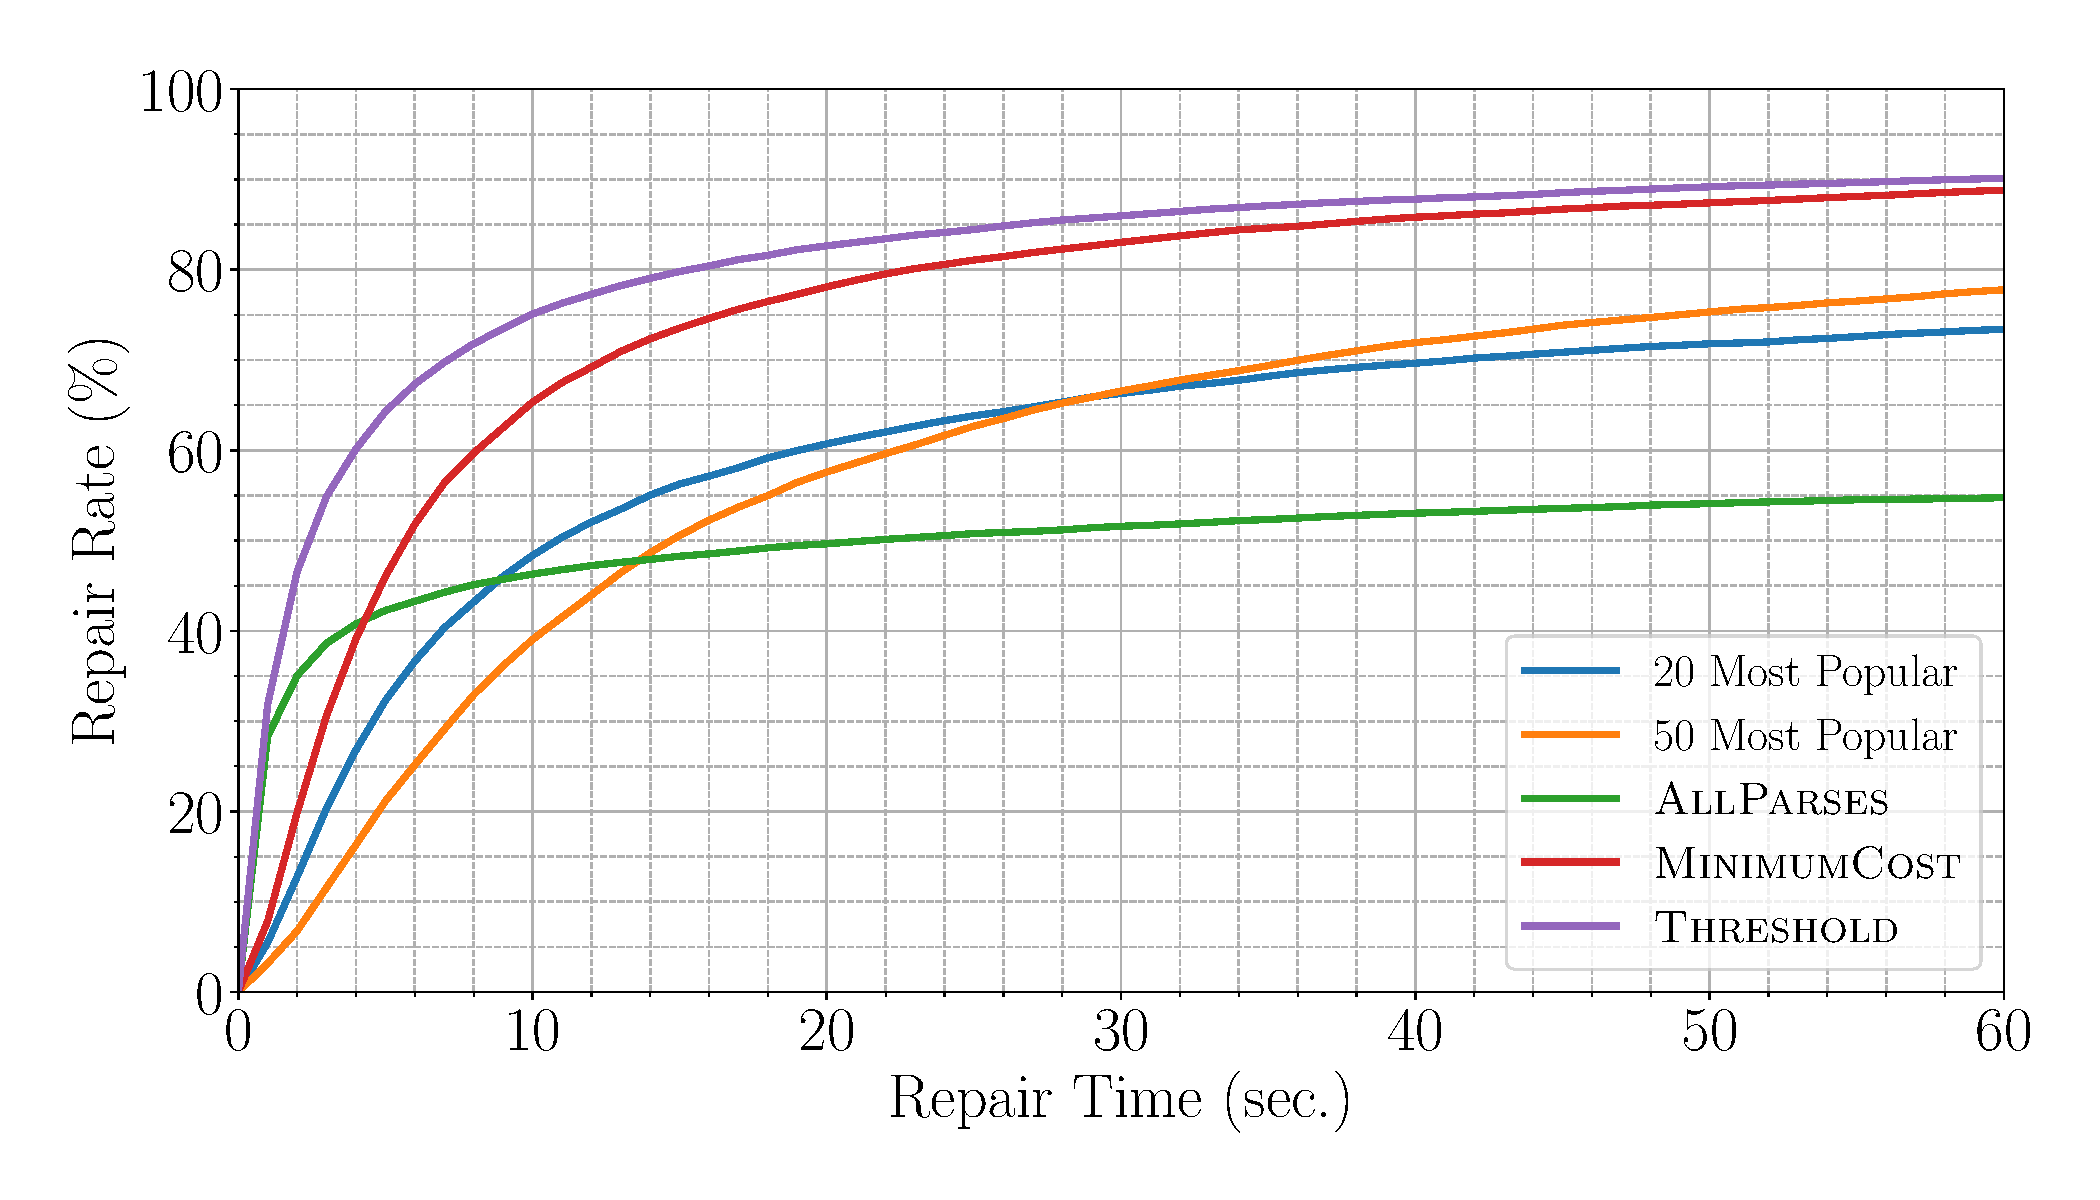
\includegraphics[width=0.85\linewidth]{tool-repair-rate.pdf}
  \caption{The repair rate for all the approaches in
  \autoref{tab:seq2parse_full_results}. \GS{\sout{TODO: Zoom out graph and
  smoothen by fitting a line over results}}}
  \label{fig:tool-repair-rate}
\end{figure}

\subsection{RQ3: Efficiency}
\label{sec:eval:efficiency}

Next we evaluate \toolname's efficiency by measuring how many programs it is
able to parse. We limit each ECE-Parser to 5 minutes. (In general, the procedure
is undecidable, and we conjecture that a longer timeout will diminish the
practical usability for developers.) We compare the efficiency of \toolname for
all the versions of \autoref{tab:seq2parse_full_results} using the full test set
of 15,000 programs.

\GS{\sout{TODO: Going to add median parse times for small/big programs and a
few/a lot syntax errors to show scalabilty. Added results below.}}

\autoref{fig:tool-repair-rate} shows the cumulative distribution function of all
\toolname approaches' repair rates over their repair time. We observe that using
\textsc{Threshold} predictions with the \textsc{MinimumCost} ECE-Parser is the
most efficient and it maintains the highest parse accuracy at all times, with a
repair rate of 83.04\% within 20 seconds and a median parse time of 2.1 seconds.
We also observe that the median parse time for \emph{larger programs} is
slightly higher with 7.0 seconds for programs with more than 100 tokens and
increases a bit more for more than 500 tokens, with 10.8 seconds. While the
ECE-parser used dynamic programming may not scale greatly for larger programs,
\toolname's scalability is \emph{mostly} proportional to the predictor error
rules and the number of syntax errors.

The \textsc{MinimumCost} with the top 20 error rule predictions is still very
efficient with a repair rate of 78.10\% within 20 seconds and a median parse
time of 5.3 seconds. For larger programs the median parse time is 12.9 seconds
for programs with more than 100 tokens and 50.8 seconds for more than 500
tokens. We observe that a fixed-length set of predicted error rules can hinder
the ECE-parser, when inaccurate predictions are involved.

We observe that, using a fixed set of the 20 and 50 most popular rules,
\toolname (with the \textsc{MinimumCost} ECE-Parser) repairs 61.41\% and 58.61\%
of the programs respectively within 20 seconds, and has median parse times of
7.0 and 13.6 seconds respectively. The 50 most popular rules admit parsing fewer
programs quickly than the 20 most popular.

We also observe that \toolname successfully parses around 38.50\% of the
programs with its \textsc{AllParses} approach in 20 seconds and has a median
parse time of 23.2 seconds. While this approach is much less efficient that the
others, it is also able to generate the exact human repair in 1 out of 3
cases, representing a valuable quality tradeoff (\S~\ref{sec:eval:precise}).

\begin{framed}
  \noindent \toolname can parse programs with syntax errors for the vast
  majority of the test set in under 20 seconds with a median parse time of 2.1
  seconds.
\end{framed}

\subsection{RQ4: Usefulness}
\label{sec:eval:useful}

% FIXME - define word for non-equivalent repairs

As \toolname is intended as an aid for programmers (especially novices) faced
with parse errors, we are also interested in subjective human judgments of the
quality and helpfulness of our repairs. Around 34\% of repairs produced by
\toolname using its \textsc{AllParses} approach are identical to the historical
human repair and thus likely helpful for programmers. However, it may be that
\toolname's parses (and thus repairs) are still helpful for debugging even when
they differ slightly from the human repair (\ie \textit{non-equivalent}
repairs). To investigate this hypothesis, we conduct a human study of the
quality and debugging helpfulness of \toolname's non-equivalent repairs.

\mypara{Human Study Setup} We recruited participants from two large public
research institutions (UC San Diego and University of Michigan) and through
Twitter. The study was online, took around 30 minutes, and participants could
enter a drawing for one of two \$50 awards. In the study, participants were each
asked to rate 15 debugging hints randomly selected from a corpus of 50
stimuli.\footnote{All human study stimuli are included in our replication
package at \url{https://github.com/gsakkas/seq2parse} and via the human study
website
\href{https://dijkstra.eecs.umich.edu/~endremad/APR_HumanEval/}.}

We created the stimuli by selecting 50 buggy programs from our test set for
which \toolname and the human produced different fixes. Other than ensuring a
wide array of difficulty (as assessed by how long the human took to fix the
error), programs were selected randomly. Each stimulus consisted of a buggy
program, its associated syntax error message, and a potential program fix
presented as a \emph{debugging hint}. For each stimulus, we produced two
versions: one where the debugging hint was generated by \toolname and one where
the debugging hint was the historical human fix. Note that, in practice, the
historical human fix would \emph{not} be available to a struggling novice
in real situations: it represents future or oracular information. Informally, in
our comparison, the historical human fixes can be viewed as an upper bound.

Participants rated the quality and
helpfulness of each debugging hint using a 1--5 Likert scale. They also indicated
if the debugging hint provided helpful information beyond that in the Python
error message.
%\footnote{In this study, we used error messages from Python 3.10. Compared to earlier Python versions, 3.10 includes improved error messages for Syntax Errors.}.
Participants were unaware of whether any given hint was generated by a human or
\toolname, and participants were never shown multiple
fixes to the same program. To be included in the analysis, participants
had to assess at least four stimuli. Overall, we analyze 527 unique stimuli
ratings from $n=39$ valid participants (246 for human fixes and 281 for
\toolname).

\mypara{Overall Results} While humans in our study find that non-equivalent
repairs produced by \toolname are lower in both quality and debugging
helpfulness than those produced manually (2.9/5 helpfulness for tool-produced
repairs vs. 3.7/5 for human-produced repairs, $p < 0.001$), humans still often
find \toolname's fixes helpful for debugging. Participants found that \toolname
repairs contained helpful debugging information beyond that contained in the
Python Error message 48\% of the time (134/281). This additional debugging
information was helpful in terms of both the content (73\% of the time) and
location (55\% of the time). Additionally, \toolname fixes are helpful for easy
and hard Syntax Errors alike: we found no statistically-significant difference
between the helpfulness or quality of \toolname's repairs for easy (those
repaired by the human in under 40 seconds) or hard parse errors (over 40
seconds).
%p = 0.07 and 0.13 respectively if we have room to include
Overall, these results indicate that even when \toolname repairs differ from
historical human repairs, they can still be helpful for debugging.

\mypara{Individual Stimuli} Beyond an analysis of \toolname's overall quality, we also
analyze the helpfulness of each stimulus. % FIXME: If room, can add more statistical details if needed
Of the 48 programs for which we collected sufficient data to permit statistical
comparison, the historical repair was statistically more helpful for debugging
than \toolname's repair for 33\% of stimuli (16/48, $p<0.05$). However, we found
that \toolname's repair was actually \emph{more helpful} for debugging than the
human's repair for 15\% of stimuli (7/48, $p<0.05$). For the remaining 52\% of
stimuli, we found no evidence of a statistical difference in the debugging
helpfulness of the two repairs.

\begin{figure}[t]
  \centering
  \begin{minipage}[c]{0.47\linewidth}
  \begin{python2}
# Buggy
def gcdIter(a, b):
    for i in range(1, a+1):
        if a % i == 0:
        elif b % i == 0:
    return i
gcdIter(9, 12)
  \end{python2}
  \begin{python2}
# Human
def gcdIter(a, b):
    for i in range(1, a+1):
        return a % i
gcdIter(9, 12)
  \end{python2}
  \begin{python2}
# Seq2Parse
def gcdIter(a, b):
    for i in range(1, a+1):
        if a % i == 0: new_var
        elif b % i == 0: break
    return i
gcdIter(9, 12)
  \end{python2}
  \subcaption{\toolname repair significantly more helpful:
  4.3/5 vs 1.0/5, $p = 0.03$}
  \label{fig:proga}
  \end{minipage}%
  \hspace{0.02\linewidth}%
  \begin{minipage}[c]{0.47\linewidth}
    \begin{python2}
aList = [12, 'yz', 'ab'];
aList.reverse();
print "List : ", aList
    \end{python2}
    \begin{python2}
aList = [12, 'yz', 'ab']
aList.reverse()
    \end{python2}
    \begin{python2}
aList = [12, 'yz', 'ab']
aList.reverse()
print("List : ", aList)
    \end{python2}
    \subcaption{\toolname repair significantly more helpful:
    4.75/5 vs 2.0/5, $p = 0.02$}
    \label{fig:progb}

    \begin{python2}
a = int(input(enter a))
print(a***3)
    \end{python2}
    \begin{python2}
a = int(input("enter a"))
print(a**3)
    \end{python2}
    \begin{python2}
a = int(input(enter)(a))
print(a ** (* 3))
    \end{python2}
    \subcaption{Historical human repair significantly more helpful:
    1.8/5 vs 4.75/5, $p = 0.01$}
    \label{fig:progc}
    \end{minipage}%

  \caption{Three example buggy programs followed by their historical human
  and \toolname repairs. For (a) and (b), \toolname's repair
  was rated more helpful by participants. For (c), the human
  repair was more helpful.}
  \label{fig:user_study_examples}
\end{figure}

To better contextualize these results, we provide examples of stimuli with
statistically significant differences in debugging helpfulness.
In figure~\ref{fig:progb}, \toolname's repair was
significantly more helpful than the historical repair:
 \toolname correctly adds parentheses to \texttt{print}
while the human simply deletes the
buggy line, perhaps out of confusion or frustration.
Similarly, figure~\ref{fig:proga}'s \toolname repair was also
better than the human repair. In this case, the user appears to try to
implement a function to calculate the greatest common divisor of two integers,
but has empty \texttt{if} and \texttt{elif} statements.
To ``fix'' this bug, the user
deletes the \texttt{if} and \texttt{elif} and modifies the return statement.
However, this fix does not correctly calculate the greatest common divisor.
\toolname, on the other hand, adds a template variable to the \texttt{if} and
\texttt{break} to the \texttt{elif}. While this also does not implement
greatest common divisor, it is viewed as more helpful
than the user repair. This example also demonstrates the beneficial ability of our approach
to conduct multi-edit repairs.

Figure~\ref{fig:progc}, on the other hand, shows an example of a more
helpful human repair. In this case, the
human correctly deletes the extraneous \texttt{*} in the power operator
while \toolname adds parentheses to make a more complex expression, the
result of favoring one insertion over one deletion.

\begin{framed}
  \noindent
  34\% of \toolname's repairs are equivalent to historical repairs.
  Of the remainder, our human study found 15\% to be more useful than
  historical repairs and 52\% to be equally useful. In total, including
  both equivalent and non-equivalent cases, \toolname repairs are at
  least as useful as historical human-written repairs 78\% of the time.

  % Even when non-equivalent, \toolname's repairs are still useful and helpful:
  % they contain debugging information beyond that in the Python error message 48\% of the time.
  % Ultimately, two-thirds of \toolname's fixes were either indistinguishable
  % from (34\%), or judged better than (15\%), those produced by humans for helping debugging.
\end{framed}
